\documentclass[10pt, a4paper]{report}

\usepackage[german,ngerman]{babel}
\usepackage{fontspec}
\usepackage{graphicx}

\begin{document}
		\begin{center}
		\huge \textbf{Softwareentwicklungspraktikum Spieleentwicklung mit JavaScript}\\
		\vspace{1cm}
		\small 
		\textbf{Daniel Bartesch, Karl Ischebeck, Philipp Koch, Janina van Rinsum}	\\
		\textbf{Sebastian Mader}									\\
		\textbf{SoSe 2019}											\\
		\textbf{LMU München}
		\vspace{1cm}
	\end{center}
	\section{Aktueller Stand und Finalisierung der Spielidee}
	Zum aktuellen Zeitpunkt hat sich die Gruppe mit dem Lehrmaterial eingehend beschäftigt und hat bereits das zentrale Projekt weitestgehenst geplant. Die Spielidee des Projekts ist eine Neuimplementierung des Game-Klassikers \textit{Bomberman}. Dazu soll über einen objektorientierten Entwurf, welcher im Bereich UML-Diagramm dargestellt wird, in TypeScript implementiert werden. Die Wahl fiel deswegen auf Typescript, weil wir uns nach den bisherigen Erfahrungen mit JavaScript eine einfachere und weniger fehleranfällige Entwicklung erhoffen. \\
	\section{Modellierung des Spiels}
	Im Rahmen unseres Projektes wollen wir den Spieleklassiker „Bombermann“ implementieren. Das Grundprinzip von Bomberman besteht darin das auf einer labyrinthartigen Karte mehrere Spieler gegeneinander antreten und versuchen als Letzter übrigzubleiben. Um dieses Ziel zu erreichen müssen alle Gegenspieler mithilfe der namensgebenden Bomben ausgeschaltet werden. Jeder Spieler hat die Möglichkeit eine Bombe auf dem Spielfeld zu platzieren die nach einem kurzen Intervall in einem kreuzförmigen Muster explodiert. Befindet sich ein Gegner im Explosionsradius so nimmt dieser Schaden der mit seinen Hitpoints verrechnet wird. Sinken diese auf null so ist dieser Spieler ausgeschieden. Sobald nur noch ein Spieler im Spiel ist hat dieser die Runde gewonnen.
	\subsection{Umsetzung}
	Zuerst sollen alle grundlegenden Funktionen implementiert werden. Also das Darstellen der Spielkarte, welche aus vielen quadratischen Feldern mit unterschiedlichen Eigenschaften bestehen wird, und der Spieler sowie die Bewegung dieser innerhalb der Karte. Besonders wichtig wird das diese Bewegungen bzw. alle Aktionen von Spielern zeitgleich mit allen anderen Spielern synchronisiert werden, sodass alle Dasselbe auf ihrem Bildschirm sehen. Danach soll die Bomben hinzukommen, hierzu haben wir uns überlegt eine Bombe als einen Untertyp der Felder aus denen das Spielfeld besteht zu implementieren. Wenn der Spieler eine Bombe legt wechselt das Feld auf dem er steht seinen Typ zu einem Bombenfeld, explodiert und wird danach wieder zu einem normalen passierbaren Feld. Geplante Feldarten sind: 
	\begin{itemize}
		\item Mauerfelder, welche den äußeren Rand der Karte abgrenzen, sowie innerhalb der Karte die Labyrinthstruktur bilden
		\item Freie Felder welche frei passierbar sind und auf denen Bomben gelegt werden können
		\item Zerstörbare Mauerfelder, die verschwinden falls sie von einer Bombenexplosion erfasst werden und damit den Typ wechseln
		\item Löcher in die die Spieler fallen können
		\item Felder auf denen benutzbare Gegenstände liegen
	\end{itemize}
	Zu diesen benutzbaren Gegenständen gehören unter anderem:
	\begin{itemize}
		\item Schilder welche die Hitpoints eines Spielers erhöhen
		\item Tränke welche die Hitpoints eines Spielers regenerieren
		\item Tränke welche die Bewegungsgeschwindigkeit des Spielers erhöhen
		\item Spezielle Bomben die z.B. einen größeren Explosionsradius haben
		\item Mauern die aufgestellt werden können um den Gegenspielern den Weg abzuschneiden
	\end{itemize}
	Weiter mögliche Features:
	\begin{itemize}
		\item Zufallsgenerierte Karten
		\item Mehr Items
		\item Mehr Feldarten
		\item Ranglisten
	\end{itemize}
	\subsection{UML-Diagramm}
	Die Planung, welche aktuell die Implementation des Spiels betrifft, soll im folgenden UML-Diagramm dargestellt werden. Das Spiel soll in verschiedene Klassen aufgeteilt werden, wobei die Klasse \textit{Game} die zentrale Klasse darstellt. Weiterhin werden die Spieler in einer eigens vorgesehenen Klasse \textit{Player} verwaltet. Diese sind auf einem Array in der Klasse Game gespeichert. Für die korrekte Darstellung des Spielzustandes, soll auch eine Klasse \textit{Field} mit verschiedenen Kindklassen implementiert werden. Hier ist das Ziel die Objekte auf dem Spielfeld verallgemeinbar zu machen. Dazu soll eine Klasse \textit{Bomb} abgeleited werden, die Bomben im Spiel darstellt und innerhalb der Spiellogik diese hinsichtlich ihrer explodierenden Eigenschaft verwaltet. Ebenfalls sollen Wandteile mithilfe einer weiteren Kindklasse von \textit{Field} über die Klasse \textit{Wall} dargestellt werden können. Mithilfe der objektorientierten Herangehensweise wird eine höhere Flexibilität hinischtlich des Gamedesigns erhofft, sodass verschiedene Temmplates leichter ausgetauscht werden können und in verschiedenen Spielständen das Feld ein unterschiedliches visuelles Design aufweisen kann.\\
	Eine weitere Planung wird den Items, die im Spiel benötigt werden gewidtmet. So sollen über eine eigens spezifizierte Klasse \textit{Item} verschiedene Eigenschaften den Spielern ermöglicht werden, welche über die Methode performAction() innerhalb der Klasse \textit{Item} aufgerufen werden können. Mithilfe der Items soll der Spieler besondere Attribute erhalten, die im Spielverlauf vorteilhaft sein können. Im weiteren Verlauf sollen Kindklassen der Klasse \textit{Item} gebildet werden, die zum aktuellen Zeitpunkt noch nicht näher spezifiziert wurden.
	
	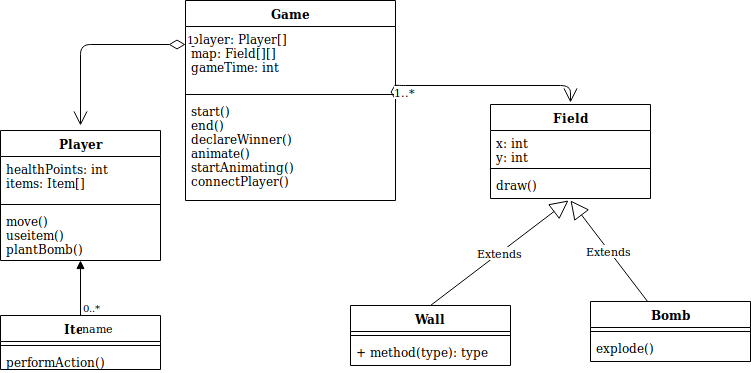
\includegraphics[scale=0.4]{UML.png}]
	
	\subsection{Herausforderungen und erwartete Probleme}
	Zunächst werden wir uns eingehend mit TypeScript befassen müssen und weiterhin die Technik um Node.js näher erlernen müssen. Dazu müssen wir gerginfügig mehr Zeit einplanen, sodass hier kein Zeitstress den Meilensteinplan ausser Kraft setzen kann. Wie sich bereits in bisherigen Projekten zeigte, kann auch die Arbeit mit Git problematisch sein, worauf wir besonders achten müssen.
	\section{Meilensteine}
	Das Projekt soll ab dem 21. Mai 2019 beginnen. Um den Entwicklungsplan einhalten zu können, werden im folgenden Meilensteine aufgestellt, die eine Oriientierung für
	die Entwicklungsphasen bieten. 
	\begin{itemize}
		\item 21.05.2019 - 11.06.2019 Implementierung der Spiellogik, Klasssendiagramm als Grundlage
		\item 11.06.2019 - 02.07.2019 Multiplayer, Verschiedene Items
		\item 16.07.2019 - 23.07.2019 Visuelle Designanpassung, Testen
	\end{itemize}
\end{document}